\chapter{Representative State Transfer (REST)}
\label{chap:rest}

\lstset{frame=none,
  language=JAVA,
  aboveskip=3mm,
  belowskip=3mm,
  showstringspaces=false,
  columns=flexible,
  basicstyle={\small\ttfamily},
  numbers=none,
  breaklines=false,
  breakatwhitespace=false,
  tabsize=3
}

\section{REST architecture}
\label{sec:rest-architecture}

The REST is "a set of constraints on the overall architectural approach" \cite{agile-architecture}. Roy Thomas Fielding described a REST in his doctoral dissertation as an architectural style. The constraints are applied to the architecture to obtain desired properties of developed architecture. REST is applicable to \gls{hypermedia}  applications where multimedia nodes are connected via hyperlinks.

REST architecture is client-server. The server holds implemented logic of services and encapsulates it under the interfaces. The interfaces are entry points for client and through them he can obtain or modify the data. TODO obrazok

The REST style is resource based \gls{resource-based-model}, it handles with resources named by nouns and actions are provided by HTTP requests. 
REST architecture is a composition of elements, connectors and components. None of them defines concrete technology, they are abstractions. The elements abstract a behaviour of components. The components have its roles, the way of interaction among them and interpretation. These elements will be described in section \ref{sec:rest-composition}

REST has its best practices and constraints. Just services which are built according to this definition can be called \emph{RESTful}. There are 6 constraints characterizing the REST which will be described further in this chapter \ref{sec:constraints}.

\section{Composition of REST}
\label{sec:rest-composition}
As has been mentioned above REST architectional style consist from data elements, connectors and components. REST is resource-based so the main data element is resource, it is accompanied by resource metadata, then the REST consists of represenatation which has its metadata. The last part od data elements are control data. Then there are connectors and components.

\subsection{Data elements}
\subsubsection{Resource}
  Resource is an abstraction of information, where any information which can be named by noun can be a resource. "A resource is a conceptual mapping to a set of entities.." \cite{fielding} or set of values. The values can be a resource identifier and a representation.
  Resource can be static, for example \emph{an image}, or dynamic, \emph{the time} which dynamically changes.
  
  Examples:
  \begin{center} 
  \begin{lstlisting}
      customer, 
      account, 
      order, 
      ..
  \end{lstlisting} 
  \end{center}

\subsubsection{Resource identifier}
  It serves to identify resources which interact with components. The resource identifier is assigning the name thanks to which it is possible to reference appropriate resource. The identifier is \gls{uri}, it marks a path to reach the resource. A request form client is routed to the specific address and method which is asked to be performed. 
There should be possible to perform the \gls{CRUD} operations with the resources, every operation can be mapped on HTTP method. Having the method and the path the specific operation is performed.


Examples: \\
\begin{center}
\begin{tabular}{l l l}
Method & URL Path & Operation performed \\ \hline
GET & /customers & Retrieves all customers \\
GET & /customers/5 & Retrieves customer with id 5 \\
POST & /accounts & Creates new account \\
PUT & /accounts/13 & Updates account with id 13 \\
DELETE & /customer/2 & Deletes customer with id 2 \\
\end{tabular}
\end{center}

\subsubsection{Representation}
  Representation is used by REST components to perform changes to the resource. Format of representations data is called media type and have influence on the performance of the hypermedia. Media types can be proprietary or standardized, from standardized types there are for comparison \gls{xml} and \gls{json}. JSON format is less verbose than XML and in consequence in sake of data transmission it would be performed faster than a XML representation format.
  
Example of representation:
\begin{center}
  \begin{tabular}[b]{l l}
    In XML format & \begin{lstlisting}
    <?xml version="1.0" encoding="utf-8">
    <customer> 
      <name>Peter<\name> 
      <surname>Smith<\surname> 
      <dateofbirth>20-4-1975<\dateofbirth> 
    <\customer>
    \end{lstlisting} \\
    
    
    In JSON format & \begin{lstlisting}
    {
        "name": "Peter", 
        "surrname": "Smith", 
        "dateofbirth": "20-4-1975"
    }
    \end{lstlisting}
  \end{tabular}
\end{center}

\subsubsection{Representation metadata}
  This metadata describes the data of which the representation consists of.
  
  Examples: \hfill \\
  \begin{center}
  \begin{lstlisting}
    {Content-Type: text/plain} 
    {Content-Type: text/xml}
  \end{lstlisting}
  \end{center}
  
\subsubsection{Resource metadata}
  Resource metadata stores an information about the resource that is not specific to the supplied representation.
  
  Example: 
  \begin{center}
  \begin{lstlisting}
    {Allow: GET}
  \end{lstlisting}
  \end{center}
  
\subsubsection{Control data}
  Control data describes the purpose of a message between components, for example \emph{GET} and parametrizes the request, for example to define cacheability. 
  
\bigskip

  Every resource has its representation, it describes how resources get manipulated in RESTful \gls{api} architecture. The representation represents part of (or less commonly the whole) resource state, it is transferred between the client and server and has generally the JSON or XML format, but could be in many other formats as well. The representation is composed from resource and attached files which provide enough information for the client to be able to modify the resource on the server.

\subsection{Connectors}
The connectors provides the access point for the values of the resource. In connectors belong client, server, cache, resolver, tunnel. %TODO explanation, maybe image

\subsection{Components}
REST components are an abstraction of application unit. The components are origin server, gateway, proxy, user agent. %TODO explanation, maybe image

\section{REST constraints}
\label{sec:constraints}

The REST architectural style has to be developed respecting its constraints. They are applied to an architecture to create RESTful services. This rules leads to desirable properties of the system, such as performance, scalability, simplicity, modifiability, visibility, portability and reliability. Constraints described below was defined by Roy Thomas Fielding and there are six of them in total:
%%(citacia http://www.restapitutorial.com/lessons/whatisrest.html#)
 
%TODO write about HATEOAS

\subsection{Uniform Interface}
  
Interface stands between client and server. Through the interface client enters server. The REST interface is uniform, client and server always use a fixed set of verbs to provide operation over the resources. REST uses \emph{\gls{http} specification}, mostly GET, POST, PUT and DELETE verbs. Despite REST can work with other protocols and define different verbs it uses HTTP operations for practical purpposes. This concept than separates client and server allowing them to develop each part independently and reducing the coupling between them. %The interface is uniform, so that is easy to understand for both, the server and the client.

Interface is resource-based. Resources are on the server side and the client sents a request to proceed the create, get, update or delete operation over the resource. The request contains a resource identifier in \gls{uri}, it identifies a path to concrete resource. Depending on the type of request the represention is sent from the client in request and/or from the server in response. The representation is conceptually separated from the resource and is commonly in XML or JSON format. It represents appropriate database record.

Resources are manipulated exclusively through the representations. The representation with any metadata attached keeps enough information for the client and allow him to modify the resource on the server.

%Sent message represents a clients request or a servers response and it is self-descriptive. It means there is enough information to know how to process the message and the response explicitly defines the cashability.

The representation is sent using HTTP verbs (GET, POST, PUT, DELETE,..) and the URI, server sends to the client the HTTP response.

\subsection{Stateless}
  
Each message is self-descriptive, a request has enough context to be understand and the messages have no state. Any state of a \gls{session} is held just on the client side. For example a logged-in user's session.
The statelessness allows greater scalability, because server doesn't have to communicate with the session, which can be created to carry the state using another architectural style of services. Reliability is improved because of easier recovery of partial failures. Disadvantage is that the sent requests contain repetitive data and the server has lower control over the application behaviour.

\subsection{Client-server}

RESTful architecture is client-server oriented. There are two disconnected concerns, it is properly defined what is consumer's side and what are services on server side. Client can’t have direct access to the database, assets or resources. Client-server architecture improves portability of both client and server codes because they are standing alone. The architecture provide simplicity and scalability of server-side code because it doestn't have to include user interface. Client and server are linked together thanks to uniform interface and the two concerns can be developed independently.

\subsection{Cacheable}

Server responses (representations) are cacheable, everything that comes back to server or from REST service could be cacheable. Responses are able to to define themselves as cashable implicitly, explicitly or negotiated. The cache can be established on server-side, client-side or both as can be seen on Figure \ref{fig:cacheability}. The reason for cacheing is to reduce interactions over the network, the cached responses are loaded from the cache instead of operating sent request. %The client-side cacheing is explained by Figure \ref{fig:clinet-side-cache}. 
Cacheing partially limits the client-server interaction but improves the scalability and performance. 


\begin{figure}[htp] \centering{
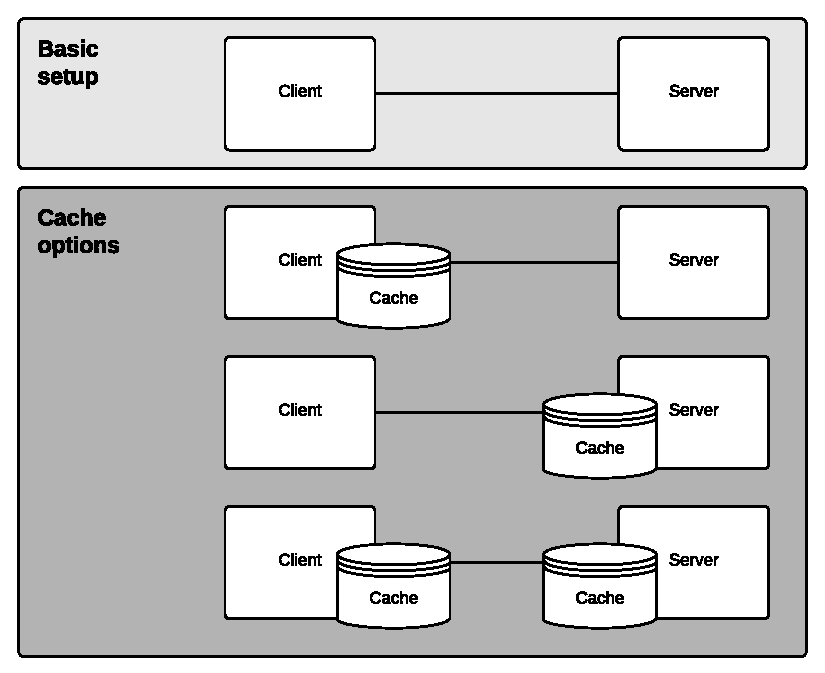
\includegraphics[width=10cm]{img/cacheablity.pdf}}
\caption{Cacheability options}
\label{fig:cacheability}
\end{figure} 

\subsection{Layered system}

A constraint inked to cashability and client-server principle. System is composed by layers which rapresents independent part of the system. Example of vetically layered system is shown on Figure \ref{fig:layered-system} Client is not able to see if he is communicating directly with the server, or with an intermedia between them. Intermedia improves scalability, provide shared caches and moreover can enforce the security policies.

\begin{figure}[htp] \centering{
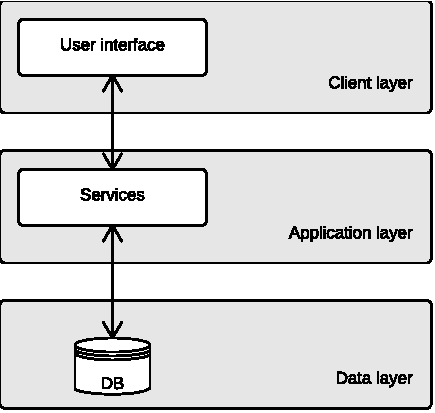
\includegraphics[width=7cm]{img/layered-system.pdf}}
\caption{Layered system example}
\label{fig:layered-system}
\end{figure} 

\subsection{Code on demand}

The logic can be transferred on the client-side, this way the server can temporarily extend or customize the functionality of the client. This can be performed for example by the components like service-side scripts.
This constraint is unique, it is the only one which can be violated and the services can be still RESTful.

\section{Application of REST}

Having the SOA and knowing the constraints of the REST services can be designed. When a company wants to develop a system with RESTful services it has to apply at least the first five of constraints. But it can occur that not all the constraints are profitable for an application. In this case the architecture can forget some of them but the services cannot be further marked as RESTful. This notation doesn't affect services themselves, the result can be still the best design for current application. The RESTful services and their constraints are one of the possible resolutions of architectural style. They are not the universal solution for system architecture.

\subsection{RESTful service example}
There is a corporation with SOA and its services are designed according to REST constraints. One of the services is representing business abstraction of \emph{customers} of the company. Customers can be viewed, created, modified or deleted. The HTTP verbs (GET, POST, PUT, DELETE) are used to perform the operations. 

In designing the service there is considered the notation of \gls{webapi} \gls{framework}. 

Resource identifier is a \gls{uri} address. ASP.NET Web API is composed of \emph{controller} and an \emph{action}. The controller is a class handling the HTTP request and the action is a method of the controller. In this example the controller is \emph{customers}, the action can be \emph{GET} and to identify a specific customer the parameter \emph{name} as to be a part of URI.

\begin{lstlisting}
    GET     customers/getByName/{name} 
\end{lstlisting}

When the client wants to get the customer whose name is \emph{Peter} then the request looks like:

\begin{lstlisting}
    GET     customers/getByName/Peter 
\end{lstlisting}

Thanks to URI the request is routed to specific resource and returns a response. In this response is a representation containing customer identified by requested name. Representation has its media type which are stated in the metadata in this  example it's JSON format:

\begin{lstlisting}
    { 
    "name": "Peter",
    "surname": "Sun",
    "e-mail": "peter.sun@service.com" 
    }
\end{lstlisting}

When the number of customers increases it is not hard to realize that the name identifier is not sufficient. There might be more than just one of the customer named "Peter". The name is obviously not unique and the best solution how to identify an entity is to assign it unique \emph{id} identifier. 

The request and response than look like:
\begin{lstlisting}
    GET     customers/getByName/{id} 
    
    GET     customers/getByName/2 
    
    { 
    "id": 2,
    "name": "Peter",
    "surname": "Sun",
    "e-mail": "peter.sun@service.com" 
    }
\end{lstlisting}


In case the service from the example above is already released and used by client a change can be done. The need of changes like this one is seriously affecting server and client and it is necessary the change is implemented by both of them. How to handle them is a main topic of this thesis and will be explained and analysed in the rest of this work.




